% =============================================================================
%  Lineage-Aware Memory Governance for Enterprise AI Agents
%  IEEE Access submission format --- official ieeeaccess/IEEEtran template
%  Full derivations, walkthroughs, and raw tables in the Supplementary Material
% =============================================================================
\documentclass[nolineno]{ieeeaccess}

% ── Language ──────────────────────────────────────────────────────────────────
\usepackage[T1]{fontenc}
\usepackage[utf8]{inputenc}
\usepackage[english]{babel}

% ── Core typesetting ──────────────────────────────────────────────────────────
\usepackage{amsmath,amssymb,amsthm}
\usepackage{mathtools}
\usepackage{graphicx}
\usepackage{booktabs}
\usepackage{array}
\usepackage{multirow}
\usepackage{xcolor}
\usepackage{pifont}
\usepackage{tcolorbox}
\tcbuselibrary{listings,breakable,skins}
\usepackage{listings}
\usepackage{tikz}
\usetikzlibrary{arrows.meta,positioning,fit,shapes.multipart,calc}
\usepackage[hidelinks,
            pdftitle={Lineage-Aware Memory Governance: A Derivation-Gated
                      Framework for Privacy-Preserving Column-Level Access
                      Control in Enterprise AI Agents},
            pdfauthor={Venkata Sangaraju; Sudhir Vissa},
            pdfkeywords={lineage-aware memory governance,enterprise AI agents,
                         privacy-preserving retrieval,column-level access control,
                         multi-agent systems,data provenance,metric governance}]{hyperref}
\usepackage{cleveref}
\usepackage{xurl}
\usepackage{enumitem}
\usepackage{caption}
\usepackage{balance}
\usepackage{placeins}

% ── Let double-column (spanning) floats use more of the page ─────────────────
\renewcommand{\dbltopfraction}{0.9}
\renewcommand{\dblfloatpagefraction}{0.85}
\setcounter{dbltopnumber}{4}
\renewcommand{\topfraction}{0.9}
\renewcommand{\textfraction}{0.07}
\renewcommand{\floatpagefraction}{0.8}

\captionsetup{font=small,labelfont=bf,labelsep=period}

% ── Theorem environments ──────────────────────────────────────────────────────
\newtheorem{theorem}{Theorem}
\newtheorem{corollary}[theorem]{Corollary}
\newtheorem{definition}{Definition}
\newtheorem{assumption}{Assumption}
\newtheorem*{remark}{Remark}

% ── Pseudocode colours ────────────────────────────────────────────────────────
\definecolor{algbg}{HTML}{F8FAFC}
\definecolor{algframe}{HTML}{1E3A5F}
\definecolor{algkw}{HTML}{1D4ED8}
\definecolor{algcmt}{HTML}{6B7280}
\definecolor{algnum}{HTML}{374151}

\lstdefinelanguage{pseudocode}{
  morekeywords={for,if,else,return,true,false,and,or,not,in,to,do,
                begin,end,each,all,break,continue,of,with,not\_subset},
  keywordstyle=\bfseries\color{algkw},
  morecomment=[l]{\%\ },
  commentstyle=\itshape\color{algcmt},
  basicstyle=\ttfamily\tiny,
  lineskip=-1.4pt,
  aboveskip=0pt,
  belowskip=0pt,
  numbers=left,
  numberstyle=\tiny\color{algnum},
  numbersep=6pt,
  xleftmargin=14pt,
  framexleftmargin=14pt,
  breaklines=true,
  showstringspaces=false,
  tabsize=2,
}

\newtcblisting[auto counter]{algorithmbox}[3][]{%
  title={\textbf{Algorithm~\thetcbcounter}: #2\hfill\textit{\small#3}},
  colback=algbg, colframe=algframe, fonttitle=\scriptsize\bfseries,
  listing only, listing options={language=pseudocode},
  boxsep=1pt, top=1pt, bottom=1pt, left=1pt, right=1pt,
  before skip=3pt, after skip=3pt,
  breakable, enhanced, #1
}

% ── Colours ───────────────────────────────────────────────────────────────────
\definecolor{myblue}{HTML}{1D4ED8}

\setlength{\parindent}{1em}

\begin{document}

\title{Lineage-Aware Memory Governance: A Derivation-Gated Framework for
Privacy-Preserving Column-Level Access Control in Enterprise AI Agents}

\author{\authorrefmark{1}Venkata Sangaraju and \authorrefmark{2}Sudhir Vissa}

\address[1]{Independent Researcher (ORCID: 0009-0001-7716-1342)}
\address[2]{SAGE7 AI, Georgetown, Texas, USA (ORCID: 0009-0003-7865-0863)}

\corresp{Corresponding author: Venkata Sangaraju.}

\markboth{Sangaraju \MakeLowercase{\textit{et al.}}: Lineage-Aware Memory
Governance for Enterprise AI Agents}{Sangaraju \MakeLowercase{\textit{et al.}}:
Lineage-Aware Memory Governance for Enterprise AI Agents}

\begin{abstract}
Shared memory across enterprise AI agents creates two under-addressed
risks: leakage of sensitive data through results that were legitimately
computed yet not legitimately derivable by the requesting department, and
silent metric-definition drift when teams compute a key performance
indicator (KPI) of the same name through different logic. Existing
agent-memory systems (e.g., MemGPT, Zep, A-MEM, SSGM, Governed Memory,
Oracle AI Agent Memory) govern retrieval by content tags, ownership, and
roles, but none record how a stored result was derived, so none can detect
that a cached insight embeds a column the requester cannot see. We
introduce the Analytical Memory Unit (AMU), a memory schema that attaches a
full derivation (lineage) graph to every cached result, and a
lineage-gated retrieval policy that serves a memory hit only when the
requester is authorised to see every column touched during derivation.
Under a completeness assumption on lineage recording, we prove this policy
prevents retrieval of any result derived from a sensitive column outside
the requester's permissions, with $O(n)$ worst-case complexity. Across six
experiments, lineage-gated retrieval eliminates the cross-department
leakage that afflicts naive content-gated memory at $18.8$--$25.5\%$ of
simulated retrievals, retaining $81.5$--$82.6\%$ memory reuse at a
worst-case gating overhead of $13.8\,\mu$s. A small real-agent study with
LLM-generated SQL suggests the guarantee transfers to real agents
unchanged, with zero leaks across 9 round-trips and two conflicts surfaced
automatically. These results outline a practical governance layer for
shared agent memory that complements source-layer access control and
supports compliance with regulation such as the EU AI Act.
\end{abstract}

\begin{IEEEkeywords}
Lineage-aware memory governance, enterprise AI agents, privacy-preserving
retrieval, column-level access control, multi-agent systems, data
provenance, metric-definition governance.
\end{IEEEkeywords}

\maketitle

% =============================================================================
\section{Introduction}
\label{sec:intro}
% =============================================================================

Consider a mid-sized enterprise running separate Finance and Marketing AI
agents against a shared customer data warehouse.
Finance joins \texttt{customer\_pii} (which contains \texttt{income}) against
\texttt{transactions} to identify high-value customers, producing a segment
of 12,400 customer IDs and a count.
The result itself carries no raw personally identifiable information (PII) and no sensitivity tag, so under any
memory system that governs access by \emph{content}, it is freely cached and
served to the next agent that asks for ``high-value customers,'' including
Marketing---whose role was never granted access to \texttt{income}.
The derivation path silently violated column-level access policy, and none
of the content-gated safeguards common in current memory-sharing systems
(\S\ref{sec:related}) would notice, because the violation is invisible in
the stored value and visible only in \emph{how the value was computed}.
This is the default behaviour of the content-gated memory-sharing pattern
used by every system we survey in \S\ref{sec:related}.

\subsection{Motivation and Prior Gap}

The urgency tracks the pace of agent adoption: Gartner forecasts 40\% of
enterprise applications will embed task-specific AI agents by the end of
2026, up from under 5\% in 2025, and 31\% of enterprises already run at
least one agent in production, rising to 47\% in banking and
insurance~\cite{digitalapplied2026adoption}.
IBM's 2025 Cost of a Data Breach Report puts the global average breach cost
at \$4.44 million (\$10.22 million in the US)~\cite{ibm2025breach}, and El
Yagoubi et al.'s AgentLeak benchmark finds $68.8\%$ of privacy leakage in
multi-agent large language model (LLM) systems occurs through \emph{inter-agent channels}---messages,
shared memory, tool arguments---invisible to output-only
auditors~\cite{elyagoubi2026agentleak}.
Systems such as MemGPT~\cite{packer2023memgpt}, Zep~\cite{rasmussen2025zep},
A-MEM~\cite{xu2025amem}, Governed Memory~\cite{taheri2026governed}, SSGM
\cite{lam2026ssgm}, and Oracle AI Agent Memory~\cite{oracle2026memory}
demonstrate that shared, governed memory reduces redundant computation, but
\textbf{every current system controls access at the level of \emph{content}
and \emph{tags}, not \emph{derivation}} (\S\ref{sec:related}, Table~1): a
memory entry is labelled with an owner, sensitivity class, or role, and
retrieval is gated on whether the requester holds the matching label.
None of these systems---nor source-layer controls such as Apache Ranger or
Databricks Unity Catalog---record which tables were joined, which columns
were touched, or what filter logic produced a stored result; source-layer
controls prevent an unauthorised agent from \emph{querying} a restricted
column, but do not prevent a legitimately computed result from being cached
and later served to a different, less-privileged requester.
A second, independent failure mode compounds the first: different
departments often compute the same-named key performance indicator (KPI)
through different business
logic (e.g., a 90-day vs.\ 60-day churn window), and without derivation
tracking, shared memory silently propagates one team's definition to the
other---a phenomenon documented as semantic drift in enterprise business
intelligence (BI)~\cite{colrows2024metrics}, serious enough that Snowflake, Salesforce, dbt
Labs, BlackRock, and RelationalAI jointly launched the Open Semantic
Interchange initiative in 2025~\cite{snowflake2025osi}, though that effort
targets human-facing BI tools, not autonomous agents writing their own
queries.
Beyond the immediate efficiency-versus-leakage tradeoff, the EU AI Act
imposes explainability and risk-management obligations on high-risk AI
systems for which data lineage is a structural
prerequisite~\cite{euaiact2024}; a memory layer that can \emph{prove}, not
merely assert, that no result crossed a column-permission boundary converts
an audit question into a mechanically checkable property of the system.

\subsection{Contributions}

This paper makes four contributions.
\textbf{(1)} The \emph{Analytical Memory Unit} (AMU) schema and
\emph{lineage-gated retrieval} policy: a memory schema attaching a full
derivation graph to every stored result, and a retrieval algorithm gating
memory hits on column-level derivation permissions rather than content tags
(\S\ref{sec:design}).
\textbf{(2)} A formal safety guarantee: Theorem~\ref{thm:safety} proves that
lineage-gated retrieval prevents leakage of any sensitive column outside the
requester's permissions under complete lineage recording, with corollaries
on unsafe store contents and policy updates, and $O(n)$/$O(1)$ complexity
analysis (\S\ref{sec:formal}).
\textbf{(3)} An eight-threat model (T1--T8) delineating what the mechanism
protects against, what it does not, and the recommended production control
for each (\S\ref{sec:threat}).
\textbf{(4)} Six statistically validated experiments---two schema
configurations, a completeness-degradation study, an extended 43-pair fuzzy
conflict-detection study, microsecond runtime benchmarks, and a real-agent
integration with automatic SQL lineage extraction---quantifying the
governance-efficiency tradeoff and grounding the mechanism in a real,
open-source agent stack (\S\ref{sec:experiments}).
Full derivations, line-by-line algorithm walkthroughs, extended related-work
discussion, and complete per-experiment tables are provided in the
Supplementary Material to keep the main text within IEEE Access length
guidelines.

% =============================================================================
\section{Related Work}
\label{sec:related}
% =============================================================================

\textbf{Agent memory systems.}
Du~\cite{du2026survey} formalises agent memory as a write-manage-read loop.
MemGPT~\cite{packer2023memgpt} pages an LLM between a bounded context and an
external store; Zep~\cite{rasmussen2025zep} adds dual-axis temporal
knowledge-graph timestamping; A-MEM~\cite{xu2025amem} builds
Zettelkasten-style linked notes.
All three are state of the art for conversational or task-level memory, but
none model the provenance of a computed analytical result.

\textbf{Governed and enterprise memory.}
Governed Memory~\cite{taheri2026governed} and SSGM~\cite{lam2026ssgm}
introduce role-based access, tiered governance routing, and consistency
verification for evolving memory stores; Oracle AI Agent Memory
\cite{oracle2026memory} provides a commercially deployed governed core; and
AgentGuardian~\cite{abaev2026agentguardian} learns access-control policies
from execution traces.
Each governs access to a memory entry \emph{as a whole}---by owner, role, or
tool-call legitimacy---not to the individual columns that contributed to it,
so none can detect that a permitted entry embeds a forbidden column.

\textbf{Multi-user and multi-principal shared memory.}
Two very recent systems address adjacent problems. Collaborative
Memory~\cite{rezazadeh2025collabmem} models multi-user, multi-agent memory
sharing via bipartite user--agent--resource access graphs with per-fragment
provenance (contributing agents, accessed resources, timestamps) for
retrospective permission checks, and proves adherence to time-varying
read/write policies; like Governed Memory and SSGM, however, its policies
gate access to a memory \emph{fragment} as an atomic unit by identity and
permission graph, not by the individual source columns a computed result
embeds, so a fragment it permits can still silently carry a value derived
from a column outside the requester's grant. GateMem~\cite{ren2026gatemem}
is a benchmark rather than a memory system: it evaluates existing
memory-agent baselines for utility, access control, and active forgetting in
multi-principal shared-memory settings (medical, office, education, and
household domains) and finds that no evaluated method achieves robust
access control without sacrificing utility---an independent empirical
confirmation of the governance gap this paper targets, though its
leak-target annotations are defined at the level of \emph{shared facts},
not \emph{derivation graphs}, so it does not test column-level lineage
gating specifically. Neither system attaches a derivation graph to a cached
analytical result or gates retrieval on the columns touched to produce it,
which is the specific mechanism AMU contributes.

\textbf{Column-level security and provenance.}
Apache Ranger, Databricks Unity Catalog, and BigQuery enforce column-gated
access at the \emph{query layer}; DePLOI~\cite{subramaniam2024deploi} audits
such policies via natural-language-to-SQL (NL2SQL) translation.
The W3C PROV standard~\cite{moreau2011prov} and Herschel et
al.~\cite{herschel2017survey} model data provenance for extract-transform-load
(ETL) pipelines, and
LINEAGEX~\cite{zhang2025lineagex} extracts column-level SQL lineage with
high accuracy.
None of these fire at the point a legitimately computed result is cached and
later served to a different, less-privileged requester---the gap our AMU
schema closes by applying column-level derivation tracking to \emph{agent
memory entries} rather than raw database records.

\textbf{Privacy and security in multi-agent systems.}
AgentLeak~\cite{elyagoubi2026agentleak} shows most multi-agent leakage
occurs through inter-agent channels; OMNI-LEAK~\cite{naik2026omnileak} and
Alizadeh et al.~\cite{alizadeh2025leak} show prompt injection can exfiltrate
observed data; AuthGraph~\cite{wang2026authgraph} defends individual agents
by comparing an execution-derived provenance graph against an authorisation
graph (closest in spirit to our column-level gate, but scoped to
single-agent tool-calling rather than cross-department memory retrieval).
This literature targets communication channels and single-agent
manipulation; our work targets a complementary vector---a \emph{shared
analytical memory store} that leaks even when every communication link and
agent is individually secure (threat T8, \S\ref{sec:threat}).

\textbf{Metric-definition governance.}
Semantic-layer tools and the Open Semantic Interchange
initiative~\cite{snowflake2025osi} centralise \emph{human}-defined metrics
but provide no mechanism for detecting drift when an autonomous agent
computes a KPI through its own generated query---the gap our
\texttt{definition\_hash} conflict detector (Algorithm~\ref{alg:write})
targets.

Table~\ref{tab:comparison} summarises six governance dimensions across
representative systems: no prior system tracks column-level derivation, and
consequently none can gate retrieval on whether the \emph{requester} is
permitted to see every column that contributed to a cached result.
Extended per-system discussion appears in the Supplementary Material.

\begin{table*}[t]
\centering
\caption{Feature comparison of representative agent-memory and governance
systems against the Analytical Memory Unit (AMU). ``Role ACL'' = role-based
access-control list. \ding{51}~= supported,
\ding{55}~= not supported, \textasciitilde~= partial/indirect support.}
\label{tab:comparison}
\footnotesize
\begin{tabular}{@{}p{0.26\linewidth}p{0.11\linewidth}p{0.1\linewidth}p{0.11\linewidth}p{0.1\linewidth}p{0.11\linewidth}@{}}
\toprule
\textbf{System} & \textbf{Content tag} & \textbf{Role ACL} & \textbf{Column lineage} & \textbf{Drift detect} & \textbf{Retrieval gate} \\
\midrule
MemGPT             & \ding{55} & \ding{55} & \ding{55} & \ding{55} & \ding{55} \\
Zep                 & \ding{51} & \ding{55} & \ding{55} & \ding{55} & \ding{55} \\
A-MEM               & \ding{51} & \ding{55} & \ding{55} & \ding{55} & \ding{55} \\
Governed Memory     & \ding{51} & \ding{51} & \ding{55} & \ding{55} & \ding{51} \\
SSGM                & \ding{51} & \textasciitilde & \ding{55} & \textasciitilde & \ding{51} \\
Collaborative Memory & \textasciitilde & \ding{51} & \ding{55} & \ding{55} & \ding{51} \\
Oracle AI Agent Memory & \ding{51} & \ding{51} & \ding{55} & \ding{55} & \ding{51} \\
AgentGuardian       & \ding{55} & \ding{51} & \ding{55} & \ding{55} & \textasciitilde \\
Source-layer ACL (Ranger/Unity Catalog) & \ding{55} & \ding{51} & \textasciitilde & \ding{55} & \ding{55} \\
\textbf{AMU (this work)} & \ding{51} & \ding{51} & \textbf{\ding{51}} & \textbf{\ding{51}} & \ding{51} \\
\bottomrule
\end{tabular}
\end{table*}

\textbf{A note on source provenance.} The comparison systems in
Table~\ref{tab:comparison} are at different stages of peer review:
A-MEM~\cite{xu2025amem} appeared at NeurIPS 2025; MemGPT~\cite{packer2023memgpt}
is an unpublished but widely adopted and highly cited preprint that
established the field's dominant memory-tiering paradigm; Zep
\cite{rasmussen2025zep}, Governed Memory~\cite{taheri2026governed},
SSGM~\cite{lam2026ssgm}, and AgentGuardian~\cite{abaev2026agentguardian} are,
at the time of writing, preprints describing production or proposed
architectures rather than independently peer-reviewed evaluations (the
latter, from a Ben-Gurion University security group, does report its own
empirical evaluation on two real-world agent applications, but that
evaluation has likewise not yet been peer-reviewed); Oracle AI Agent
Memory~\cite{oracle2026memory} is documented only in vendor developer-blog
form, with no publicly available technical paper; and Collaborative
Memory~\cite{rezazadeh2025collabmem}, from Accenture's Center for Advanced
AI, and GateMem~\cite{ren2026gatemem} are, like the majority of this
comparison, unreviewed preprints at the time of writing. We include all of them
because Table~\ref{tab:comparison} compares
\emph{documented design decisions}---what each system's own description says
it tracks and gates on---rather than reported performance numbers we did not
independently verify; the governance gap we identify (content/tag-level
access control, not derivation-level) is a structural property of each
system's publicly stated design, and is unaffected by whether that design
has cleared peer review. We do not draw any comparative performance claims
from these sources, only feature-support claims, and we flag this
distinction explicitly so readers can weight the comparison accordingly.



% =============================================================================
\section{System Design}
\label{sec:design}
% =============================================================================

\subsection{The Analytical Memory Unit}

\begin{definition}[Analytical Memory Unit]
An \emph{Analytical Memory Unit} (AMU) is a tuple
$\langle \mathit{metric}, v, d, \tau, L \rangle$ where:
$\mathit{metric}$ is a metric-name string;
$v \in \mathbb{R}$ is the computed result value;
$d$ is the producing department;
$\tau$ is an integer epoch (supports time-to-live (TTL) eviction); and
$L = (s_1, \ldots, s_k)$ is a \emph{lineage graph}, each step
$s_i = (\mathit{table}_i,\, C_i,\, \varphi)$
where $C_i$ is the set of columns of $\mathit{table}_i$ accessed and
$\varphi$ is a filter-logic string.
\end{definition}

\begin{figure}[t]
\centering
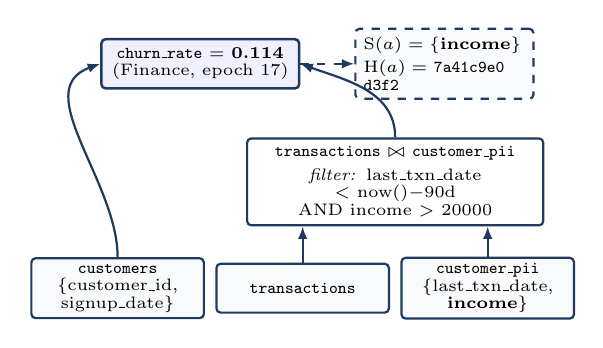
\begin{tikzpicture}[
  font=\fontsize{5.6}{6.4}\selectfont,
  leaf/.style={draw=algframe,thick,fill=algbg,rounded corners=1.5pt,
               align=center,text width=2.05cm,minimum height=0.62cm,
               inner sep=2pt},
  joinbox/.style={draw=algframe,thick,fill=white,rounded corners=1.5pt,
               align=center,text width=3.55cm,inner sep=3pt},
  resbox/.style={draw=algframe,line width=0.9pt,fill=blue!6,
               rounded corners=1.5pt,align=center,text width=2.3cm,
               inner sep=3pt},
  tagbox/.style={draw=algframe,thick,dashed,fill=algbg,
               rounded corners=1.5pt,align=left,text width=2.05cm,
               inner sep=3pt},
  arr/.style={-{Latex[length=4.5pt,width=3.5pt]},thick,draw=algframe}
]

\node[leaf] (cust) at (0,0)
  {\texttt{customers}\\\{customer\_id,\\signup\_date\}};
\node[leaf] (tx) at (2.35,0) {\texttt{transactions}};
\node[leaf] (pii) at (4.7,0)
  {\texttt{customer\_pii}\\\{last\_txn\_date,\\\textbf{income}\}};

\node[joinbox] (join) at (3.525,1.35)
  {\texttt{transactions} $\bowtie$ \texttt{customer\_pii}\\[2pt]
   \textit{filter:} last\_txn\_date $<$ now()$-$90d\\ AND income $>$ 20000};

\node[resbox] (churn) at (1.05,2.85)
  {\texttt{churn\_rate} $=$ \textbf{0.114}\\(Finance, epoch~17)};

\node[tagbox] (tags) at (4.15,2.85)
  {$\mathrm{S}(a) = \{$\textbf{income}$\}$\\[2pt]
   $\mathrm{H}(a) =$ \texttt{7a41c9e0}\\\texttt{d3f2}};

\draw[arr] (tx.north) |- ($(tx.north)+(0,0.25)$) -| (join.south -| tx);
\draw[arr] (pii.north) |- ($(pii.north)+(0,0.25)$) -| (join.south -| pii);
\draw[arr] (cust.north) to[out=90,in=200] (churn.west);
\draw[arr] (join.north) to[out=90,in=-20] (churn.east);
\draw[arr,dashed] (churn.east) to (tags.west);
\end{tikzpicture}
\caption{Worked lineage graph: Finance's \texttt{churn\_rate} is derived by
joining three source tables. Because the join touches the sensitive column
\texttt{income}, the derived tag $\mathrm{S}(a)$ makes this single cached
number unsafe to serve to any department lacking \texttt{income}
access---even though the value $0.114$ alone reveals nothing.}
\label{fig:lineage-example}
\end{figure}

Figure~\ref{fig:lineage-example} shows a worked example: the result value
$v$ alone carries no information about how it was produced; the lineage
graph $L$ makes the derivation explicit and machine-checkable at retrieval
time.
Two quantities are derived once at AMU creation and cached:
\begin{align}
  \mathrm{S}(a) &= \bigcup_{i=1}^{k} C_i \;\cap\; \mathcal{S}
  \label{eq:sensitivity} \\[2pt]
  \mathrm{H}(a) &= \mathrm{SHA256}\!\left(
    \mathrm{sort}(\mathit{tables}) \,\|\,
    \mathrm{sort}\!\left(\bigcup_i C_i\right) \,\|\, \varphi
  \right)_{\![0{:}12]}
  \label{eq:defhash}
\end{align}
where $\mathcal{S}$ is the sensitive-column registry and $\mathrm{H}(a)$ is
the \emph{definition hash} fingerprinting \emph{how} the metric was
computed.
Both are sub-microsecond in practice (\S\ref{sec:runtime}).
Table~\ref{tab:amu} lists the full schema.

\begin{table}[t]
\centering
\caption{Analytical Memory Unit (AMU) schema fields.}
\label{tab:amu}
\footnotesize
\begin{tabular}{@{}p{0.29\linewidth}p{0.63\linewidth}@{}}
\toprule
\textbf{Field} & \textbf{Description} \\
\midrule
\texttt{metric\_name}      & Business KPI name (\emph{e.g.}, \texttt{churn\_rate}) \\
\texttt{value}, \texttt{owner\_dept}, \texttt{epoch} & Result, producing department, TTL time index \\
\texttt{lineage}           & Derivation graph: sequence of $(t, C, \varphi)$ steps \\
\texttt{sensitivity\_tags} & $\mathrm{S}(a)$ (Eq.~\ref{eq:sensitivity}), cached \\
\texttt{definition\_hash}  & $\mathrm{H}(a)$ (Eq.~\ref{eq:defhash}), cached \\
\bottomrule
\end{tabular}
\end{table}

\FloatBarrier
\subsection{Lineage-Gated Retrieval and Conflict Detection}
\label{sec:algorithms}

Algorithms~\ref{alg:retrieve} and~\ref{alg:write} give the two core
operations; $\mathrm{P}(d)$ denotes department $d$'s permitted column set.
A full walkthrough of Algorithm~\ref{alg:retrieve} follows below; the
analogous walkthrough of Algorithm~\ref{alg:write} appears in the
Supplementary Material.

\begin{algorithmbox}[label={alg:retrieve}]{Lineage-Gated Retrieve}{%
  \textnormal{Input: \textit{store, metric, dept, fresh}; Output: \textit{result}; \textit{leaked}=\textbf{False}}}
candidates <- store[metric]         % all stored AMUs for this metric
permitted  <- P(dept)               % column set the department may see
blocked    <- False

for each a in REVERSE(candidates):  % most-recent-first
  if S(a) not_subset permitted:     % derivation touches a forbidden column
    blocked <- True
    continue                        % skip this candidate; try the next
  end if
  return (reused=True, value=a.value, leaked=False, blocked=False)
end for

store[metric].append(fresh)
return (reused=False, value=fresh.value, leaked=False, blocked=blocked)
\end{algorithmbox}

\begin{algorithmbox}[label={alg:write}]{Lineage-Aware Write}{%
  \textnormal{Input: \textit{store}, AMU \textit{a}; Output: \textit{conflict} \textbf{bool}}}
existing <- store[a.metric]   % all AMUs stored for this metric name
conflict <- False

for each e in existing:
  if e.dept != a.dept:        % cross-department pair
    if H(e) != H(a):          % definition hashes differ -> potential conflict
      conflict <- True
      break
    end if
  end if
end for

store[a.metric].append(a)     % always persist; conflict is surfaced, not blocked
return conflict
\end{algorithmbox}

\textbf{Line-by-line walkthrough of Algorithm~\ref{alg:retrieve}.}
Line~1 retrieves every AMU ever stored under this metric name; this list is
the candidate pool. Line~2 resolves the requester's column permission set
once, outside the loop, so it is not recomputed per candidate. Line~5
iterates candidates \emph{most-recent-first}: this is a deliberate policy
choice, not an implementation detail---it means that when a safe candidate
exists, the department receives the freshest safe value rather than an
arbitrary historical one. Line~6 is the gate: a single $O(|\mathcal{S}|)$
set-difference check (cached $\mathrm{S}(a)$ against $\mathrm{P}(d)$). If the
check fails, line~7 records that at least one candidate was blocked (used
only for diagnostics and the experiments in \S\ref{sec:experiments}) and
line~8 continues to the next-oldest candidate---the rejected candidate is
never returned, never partially returned, and never logged with its value.
Line~10 is the only successful-return statement in the loop body: it fires
the first time a candidate's derivation is fully contained in the
requester's permissions. If the loop exhausts all candidates without a safe
hit, line~13 appends the caller-supplied, already-in-scope \textit{fresh}
computation to the store (so future requests may reuse it) and line~14
returns it. Every exit path is covered by exactly one of these two return
statements, which is what the proof of Theorem~\ref{thm:safety} exploits.
\emph{Complexity:} the loop runs at most $n$ times ($n$ = candidates for
this metric), each iteration doing $O(|\mathcal{S}|)$ work, giving
$O(n\cdot|\mathcal{S}|)$ worst case; since $|\mathcal{S}|$ is a small
constant per organisation, we report this as $O(n)$ in
Table~\ref{tab:complexity}. The best case (first candidate safe) is
$O(|\mathcal{S}|) = O(1)$.

Algorithm~\ref{alg:write} compares cached definition hashes $\mathrm{H}(\cdot)$
rather than raw lineage graphs, making conflict detection $O(1)$ per pair; the
write path never blocks on a conflict, only surfaces one for downstream
alerting (threat T2). Its full line-by-line walkthrough, structurally
analogous to the one above, is given in the Supplementary Material.

\begin{figure*}[t]
\centering
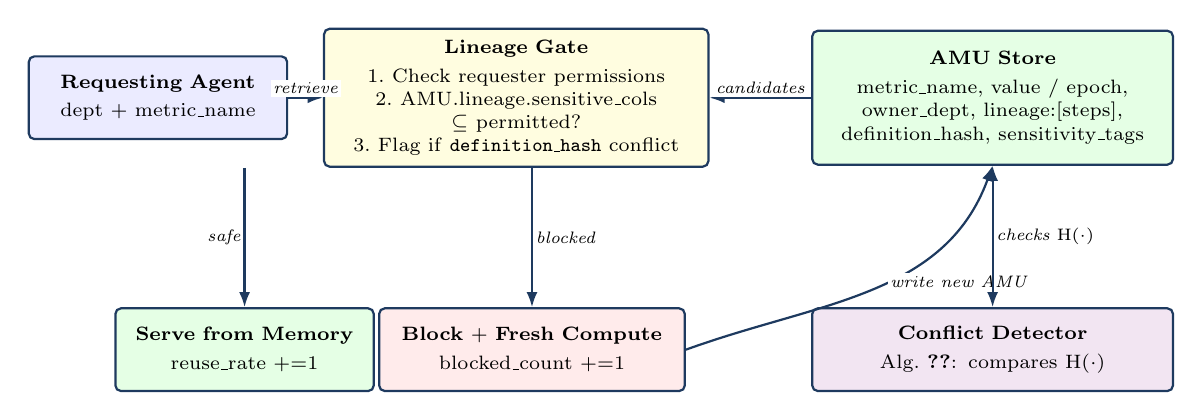
\begin{tikzpicture}[
  font=\fontsize{7.2}{8.4}\selectfont,
  every node/.style={align=center},
  agent/.style={draw=algframe,thick,fill=blue!8,rounded corners=2pt,
                text width=3.0cm,minimum height=1.05cm,inner sep=4pt},
  gate/.style={draw=algframe,thick,fill=yellow!12,rounded corners=2pt,
                text width=4.6cm,minimum height=1.7cm,inner sep=4pt},
  store/.style={draw=algframe,thick,fill=green!10,rounded corners=2pt,
                text width=4.3cm,minimum height=1.7cm,inner sep=4pt},
  serve/.style={draw=algframe,thick,fill=green!10,rounded corners=2pt,
                text width=3.0cm,minimum height=1.05cm,inner sep=4pt},
  block/.style={draw=algframe,thick,fill=red!8,rounded corners=2pt,
                text width=3.6cm,minimum height=1.05cm,inner sep=4pt},
  conflict/.style={draw=algframe,thick,fill=violet!10,rounded corners=2pt,
                text width=4.3cm,minimum height=1.05cm,inner sep=4pt},
  lbl/.style={font=\fontsize{6.4}{7.4}\selectfont\itshape,fill=white,
              inner sep=1pt},
  arr/.style={-{Latex[length=5.5pt,width=4pt]},thick,draw=algframe}
]

\node[agent]   (agent)  at (0,3.55)   {\textbf{Requesting Agent}\\[2pt] dept $+$ metric\_name};
\node[gate]    (gate)   at (4.55,3.55) {\textbf{Lineage Gate}\\[2pt]
  1.~Check requester permissions\\
  2.~AMU.lineage.sensitive\_cols $\subseteq$ permitted?\\
  3.~Flag if \texttt{definition\_hash} conflict};
\node[store]   (store)  at (10.6,3.55) {\textbf{AMU Store}\\[2pt]
  metric\_name, value / epoch,\\ owner\_dept, lineage:[steps],\\
  definition\_hash, sensitivity\_tags};

\node[serve]   (serve)  at (1.1,0.35) {\textbf{Serve from Memory}\\[2pt] reuse\_rate $+{=}1$};
\node[block]   (block)  at (4.75,0.35) {\textbf{Block $+$ Fresh Compute}\\[2pt] blocked\_count $+{=}1$};
\node[conflict](conf)   at (10.6,0.35) {\textbf{Conflict Detector}\\[2pt] Alg.~\ref{alg:write}: compares $\mathrm{H}(\cdot)$};

\draw[arr] (agent.east) -- node[lbl,above]{retrieve} (gate.west);
\draw[arr] (store.west) -- node[lbl,above]{candidates} (gate.east);
\draw[arr] (gate.south -| serve) -- node[lbl,left]{safe} (serve.north);
\draw[arr] (gate.south -| block) -- node[lbl,right]{blocked} (block.north);
\draw[arr] (block.east) to[out=20,in=250] node[lbl,right,pos=0.55]{write new AMU} (store.south);
\draw[arr,{Latex[length=5.5pt,width=4pt]}-{Latex[length=5.5pt,width=4pt]}]
  (store.south) -- node[lbl,right]{checks $\mathrm{H}(\cdot)$} (conf.north);
\end{tikzpicture}
\caption{AMU architecture. An agent's executed query is intercepted at the
database cursor and its lineage extracted (left); the AMU is written to the
shared store, where Algorithm~\ref{alg:write} checks $\mathrm{H}(\cdot)$
against cross-department entries. On the read path (right), the lineage gate
checks $\mathrm{S}(a) \subseteq \mathrm{P}(d)$ before serving from memory;
unsafe candidates are blocked and the agent falls back to a fresh in-scope
computation, itself written back through the same path.}
\label{fig:arch}
\end{figure*}

\subsection{Implementation Considerations}
\label{sec:implementation}

Three practical points arise in production deployment (details in the
Supplementary Material).
First, the cleanest integration point is the database driver layer: wrapping
the cursor so every executed SQL string passes through a lineage extractor
(\textsc{SQLGlot}, Experiment~6) means lineage capture requires zero
cooperation from the agent.
Second, the system must \emph{fail closed}: if lineage extraction fails,
treat the AMU as maximally sensitive ($\mathrm{S}(a) \leftarrow \mathcal{S}$)
rather than fail open, and if a department's permission set is unavailable,
default retrieval to denial.
Third, the \texttt{epoch} field supports both ordinary TTL eviction and
\emph{policy-driven} invalidation: when $\mathcal{S}$ or $\mathrm{P}(d)$
changes, cached $\mathrm{S}(a)$ values should be lazily recomputed on next
retrieval (Corollary~\ref{cor:policy-update}, threat T3).

% =============================================================================
\section{Formal Analysis}
\label{sec:formal}
% =============================================================================

\begin{assumption}[Complete Lineage]
\label{ass:complete}
For every AMU $a$ in the store, $a.\mathit{lineage}$ records every table,
column, and filter predicate of the computation that produced $a.\mathit{value}$.
\end{assumption}

\begin{theorem}[Sensitive-Column Safety]
\label{thm:safety}
Under Assumption~\ref{ass:complete}, Algorithm~\ref{alg:retrieve} returns no
result to department $d$ that was derived from a sensitive column
$c \in \mathcal{S}$ with $c \notin \mathrm{P}(d)$.
\end{theorem}

\begin{proof}
By inspection, Algorithm~\ref{alg:retrieve} has exactly two statements that
return a value to the caller: line~10 (memory-served) and line~14
(fallback). Every invocation terminates by reaching one of the two, since
the \texttt{for} loop either returns early at line~10 or exhausts
\textit{candidates} and falls through to lines~13--14. We show the returned
AMU's derivation touches no forbidden sensitive column on each path.

\smallskip\noindent\textbf{Case 1: memory-served path (line~10).}
Reaching line~10 for candidate $a$ requires the guard at line~6 to have
evaluated false, i.e.\ $\mathrm{S}(a) \subseteq \mathrm{P}(d)$ holds for that
$a$. Unfolding Equation~\ref{eq:sensitivity}, $\mathrm{S}(a) =
\bigl(\bigcup_{i=1}^{k} C_i\bigr) \cap \mathcal{S}$, so $\mathrm{S}(a)
\subseteq \mathrm{P}(d)$ is equivalent to: for every step $s_i \in
a.\mathit{lineage}$ and every column $c \in C_i \cap \mathcal{S}$, $c \in
\mathrm{P}(d)$. Contrapositively, there is no sensitive column $c \in
\mathcal{S}$ with $c \notin \mathrm{P}(d)$ appearing in any $C_i$---i.e., no
such $c$ appears anywhere in $a$'s derivation. Since
Assumption~\ref{ass:complete} guarantees $a.\mathit{lineage}$ records
\emph{every} column touched by the computation that produced $a.value$,
this is precisely the safety property claimed for the value returned at
line~10.

\smallskip\noindent\textbf{Case 2: fallback path (line~14).}
The input precondition to Algorithm~\ref{alg:retrieve} (stated in the
signature) requires that \textit{fresh} is computed entirely within
$\mathrm{P}(d)$ by the caller, before Algorithm~\ref{alg:retrieve} is
invoked. Under Assumption~\ref{ass:complete}, \textit{fresh}.\textit{lineage}
records every column of that computation, so every column recorded is, by
the precondition, in $\mathrm{P}(d)$; in particular no sensitive column
outside $\mathrm{P}(d)$ is touched.

\smallskip\noindent
Both cases establish that the AMU returned to department $d$ has a
derivation containing no sensitive column outside $\mathrm{P}(d)$, for an
arbitrary invocation with arbitrary \textit{store} contents. Since the two
cases are exhaustive over all return statements, the claim holds for every
invocation of Algorithm~\ref{alg:retrieve}.
\end{proof}

\begin{corollary}[Robustness to unsafe store contents]
\label{cor:unsafe-contents}
The guarantee holds even when \textit{store} contains AMUs whose derivation
touches columns outside $\mathrm{P}(d)$: such candidates fail the gate and
are skipped, regardless of how many exist or where they occur.
\end{corollary}

\begin{corollary}[Behaviour under policy updates]
\label{cor:policy-update}
The guarantee holds \emph{per policy version}: if $\mathrm{S}(a)$ is cached
under registry $\mathcal{S}_1$ and the organisation transitions to
$\mathcal{S}_2$ without recomputing existing AMUs, a column newly added to
$\mathcal{S}_2$ may not appear in the stale cached tag. The guarantee is
restored for all subsequent retrievals once $\mathrm{S}(a)$ is recomputed
against $\mathcal{S}_2$ for every AMU predating the change (formalising
threat T3).
\end{corollary}

\subsection{Complexity and Storage}
\label{sec:complexity}

Let $n$ = AMUs stored per metric, $k$ = lineage steps, $c$ = columns per
step.
Table~\ref{tab:complexity} reports asymptotic and measured costs.

\begin{table}[t]
\centering
\caption{Asymptotic complexity and measured latency (means over 2{,}000
iterations; $k{=}2$--$3$, $c{=}4$--$7$). Full runtime sweep in the
Supplementary Material.}
\label{tab:complexity}
\footnotesize
\begin{tabular}{@{}p{0.32\linewidth}p{0.12\linewidth}p{0.13\linewidth}p{0.13\linewidth}@{}}
\toprule
\textbf{Operation} & \textbf{Cplx.} & \textbf{$n{=}1$} & \textbf{$n{=}50$} \\
\midrule
Gate-check predicate        & $O(|\mathcal{S}|)$ & $0.09\,\mu$s & $0.09\,\mu$s \\
Write --- conflict detection & $O(n)$  & $0.28\,\mu$s & $1.63\,\mu$s \\
Retrieve --- worst case      & $O(n)$  & $0.66\,\mu$s & $13.82\,\mu$s \\
Retrieve --- expected case   & $O(1)$  & $0.66\,\mu$s & $0.64\,\mu$s \\
\bottomrule
\end{tabular}
\end{table}

The expected-case retrieve latency is constant regardless of store size;
the worst case (all $n$ candidates blocked) scales linearly, reaching
$13.82\,\mu$s at $n{=}50$, but in a realistic production store $n \leq 5$
(at most one AMU per department variant per metric), so both paths are
effectively $O(1)$ and well below $2\,\mu$s---negligible relative to any
real analytics query (ms--s).
The worst-case $O(n)$ bound is a deliberate design choice, not a caveat:
Algorithm~\ref{alg:retrieve} scans most-recent-first so it returns the
freshest \emph{safe} value rather than an arbitrary one; an alternative
design that indexed AMUs by $(\mathit{metric}, \mathrm{S}(a))$ could achieve
$O(1)$ worst case at the cost of extra index-maintenance complexity and the
loss of the recency-preference guarantee.
We did not adopt that design because $n$ is small by construction: a metric
name accumulates at most one AMU per distinct (department, lineage-variant)
combination, consistent with $n \leq 5$ in every workload we observed
(Experiments~1--2 and~6), at which the $O(n)$ worst case costs at most
$1.74\,\mu$s---immaterial in practice, though we report the asymptotic bound
honestly because it would matter under a poorly bounded TTL policy, which is
why we recommend TTL eviction as a standing operational control.
Relative to the $O(1)$ dictionary lookup used by all prior
systems~\cite{packer2023memgpt,rasmussen2025zep,xu2025amem,taheri2026governed,lam2026ssgm,oracle2026memory},
lineage-gated retrieval trades at most $13.82\,\mu$s in absolute terms for
the safety guarantee of Theorem~\ref{thm:safety}---a tradeoff Experiments~1--2
show buys elimination of an $18.8$--$25.5\%$ structural leak rate at a
$13$--$14$ percentage-point reuse cost.
Storage overhead is modest: an AMU adds $k$ tuples of table/column names,
the filter string, and a 12-character hash---roughly $4$--$8\times$ a bare
value entry (200--600 bytes for a typical 2--4 table join), smaller than the
SQL query most systems already persist alongside the result.

% =============================================================================
\section{Threat Model}
\label{sec:threat}
% =============================================================================

Principals are enterprise departments operating AI agents, modelled as
\emph{honest-but-potentially-over-privileged}: they request metrics they
have legitimate business need for, but not all derivation paths fall within
their column permissions.
The two threats the mechanism directly addresses motivate this work: T1
(an agent retrieves a cached result derived from a sensitive column it may
not see, mitigated by the $\mathrm{S}(a)\subseteq\mathrm{P}(d)$ gate) and T2
(two departments store conflicting definitions of the same-named KPI,
surfaced by the definition-hash conflict detector).
The most important unaddressed gap is T4, inference attacks: a derived
feature that \emph{encodes} sensitive information without naming the source
column (e.g., a risk score computed from \texttt{income}) will not be caught
unless the dependency is explicitly recorded in the lineage graph.
Table~\ref{tab:threats} summarises all eight threats; full prose
descriptions of each appear in the Supplementary Material.

\begin{table*}[t]
\centering
\caption{Threat summary. ``Addressed'' means Algorithms~\ref{alg:retrieve}--\ref{alg:write}
mitigate the threat directly under the stated assumptions; ``Partial'' means
the mechanism reduces but does not eliminate exposure; ``No'' means an
external control is required.}
\label{tab:threats}
\footnotesize
\begin{tabular}{@{}p{0.07\linewidth}p{0.44\linewidth}p{0.1\linewidth}p{0.29\linewidth}@{}}
\toprule
\textbf{ID} & \textbf{Threat} & \textbf{Status} & \textbf{Production control} \\
\midrule
T1 & Sensitive-column leakage via cached result & Addressed & Lineage gate (Alg.~\ref{alg:retrieve}) \\
T2 & Silent metric-definition drift & Addressed & Conflict detector (Alg.~\ref{alg:write}) \\
T3 & Stale sensitive data after policy update & Partial & TTL + lazy $\mathrm{S}(a)$ recompute (Cor.~\ref{cor:policy-update}) \\
T4 & Inference attacks (undeclared derived features) & No & Manual review of feature engineering; out of scope \\
T5 & Malicious/incomplete lineage fabrication & Partial & Automatic extraction (\textsc{SQLGlot}/LINEAGEX), \S\ref{sec:degradation} \\
T6 & Aggregate inference across retrievals & No & Differential privacy layer (future work) \\
T7 & Insider threats on the store & No & Trusted infrastructure, audit logging \\
T8 & Prompt injection / timing side-channel on lineage & Partial & Automatic extraction; constant-time gate (optional) \\
\bottomrule
\end{tabular}
\end{table*}

The mechanism's addressed threats (T1, T2) are exactly the two failure modes
motivating this work; the partially addressed threats (T3, T5, T8) share a
common root cause---reliance on lineage completeness and
integrity---remedied by automatic, tamper-resistant lineage extraction; and
the unaddressed threats (T4, T6, T7) mark the boundary of what a
memory-layer control can achieve without cooperation from the
feature-engineering layer, a differential-privacy layer, or the
infrastructure trust boundary.
AMU is one layer in a defence-in-depth stack, not a complete security
solution on its own.

% =============================================================================
\section{Experiments}
\label{sec:experiments}
% =============================================================================

We built a synthetic discrete-event simulator in pure Python, isolating the
retrieval-and-conflict-detection mechanism from LLM inference, network
latency, and query-optimiser confounds: every event's ground-truth lineage,
sensitivity, and department permissions are known exactly, so leak and reuse
rates are measured without label noise.
Three systems are compared: \textbf{No Memory} (leak-free, zero reuse),
\textbf{Naive Shared Memory} (content-gated, representing prior systems),
and \textbf{Lineage-Aware} (proposed).
All experiments report mean $\pm$ population standard deviation over 30
seeds, with bootstrap 95\% confidence intervals and Mann-Whitney $U$
significance tests; full protocol and raw per-seed tables are in the
Supplementary Material.

\subsection{Experiments 1--2: Synthetic and TPC-H Schemas}
\label{sec:exp1}
\label{sec:exp2}

Experiment~1 uses a 5-table synthetic schema (three departments, sensitive
columns $\mathcal{S}=\{\texttt{ssn},\texttt{email},\texttt{income}\}$, Table~\ref{tab:perms});
Experiment~2 replicates it on the 8-table TPC-H decision-support
benchmark~\cite{tpch2021} ($|\mathcal{S}_{\text{TPC-H}}|=9$) to test whether
findings generalise to a denser, more realistic schema.

\begin{table}[t]
\centering
\caption{Department permissions, synthetic schema. The gate enforces
restrictions only on columns in $\mathcal{S}$; non-sensitive blocked columns
represent full policy intent but are not currently gate-enforced.}
\label{tab:perms}
\footnotesize
\begin{tabular}{@{}p{0.16\linewidth}p{0.34\linewidth}p{0.38\linewidth}@{}}
\toprule
\textbf{Dept.} & \textbf{Permitted (summary)} & \textbf{Blocked (in $\mathcal{S}$)} \\
\midrule
Finance   & All columns            & None \\
Marketing & Commercial, order data & \texttt{ssn, income, email} \\
Support   & Customer, ticket meta  & \texttt{ssn, income, email} \\
\bottomrule
\end{tabular}
\end{table}

\begin{table}[t]
\centering
\caption{Leak and reuse rates, both schemas (30 seeds, mean $\pm$ std dev).
All naive--LA differences: bootstrap 95\% CI excludes zero, Mann-Whitney
$U$, $p<0.001$. Full tables in the Supplementary Material.}
\label{tab:combined-results}
\footnotesize
\begin{tabular}{@{}p{0.24\linewidth}p{0.15\linewidth}p{0.15\linewidth}p{0.15\linewidth}p{0.15\linewidth}@{}}
\toprule
& \multicolumn{2}{c}{\textbf{Synthetic (5-tab.)}} & \multicolumn{2}{c}{\textbf{TPC-H (8-tab.)}} \\
\textbf{Metric} & \textbf{Naive} & \textbf{LA} & \textbf{Naive} & \textbf{LA} \\
\midrule
Leak rate (\%) & $18.8\pm3.7$ & $0.0\pm0.0^\dagger$ & $25.5\pm4.5$ & $0.0\pm0.0^\dagger$ \\
Reuse rate (\%) & $95.8\pm0.0$ & $82.6\pm2.3$ & $95.8\pm0.0$ & $81.5\pm4.8$ \\
Conflict recall (\%) & $0.0\pm0.0$ & $100.0\pm0.0$ & $0.0\pm0.0$ & $100.0\pm0.0$ \\
\bottomrule
\multicolumn{5}{l}{\footnotesize$^\dagger$Formal guarantee (Theorem~\ref{thm:safety}), not an empirical discovery.}
\end{tabular}
\end{table}

\begin{figure}[t]
\centering
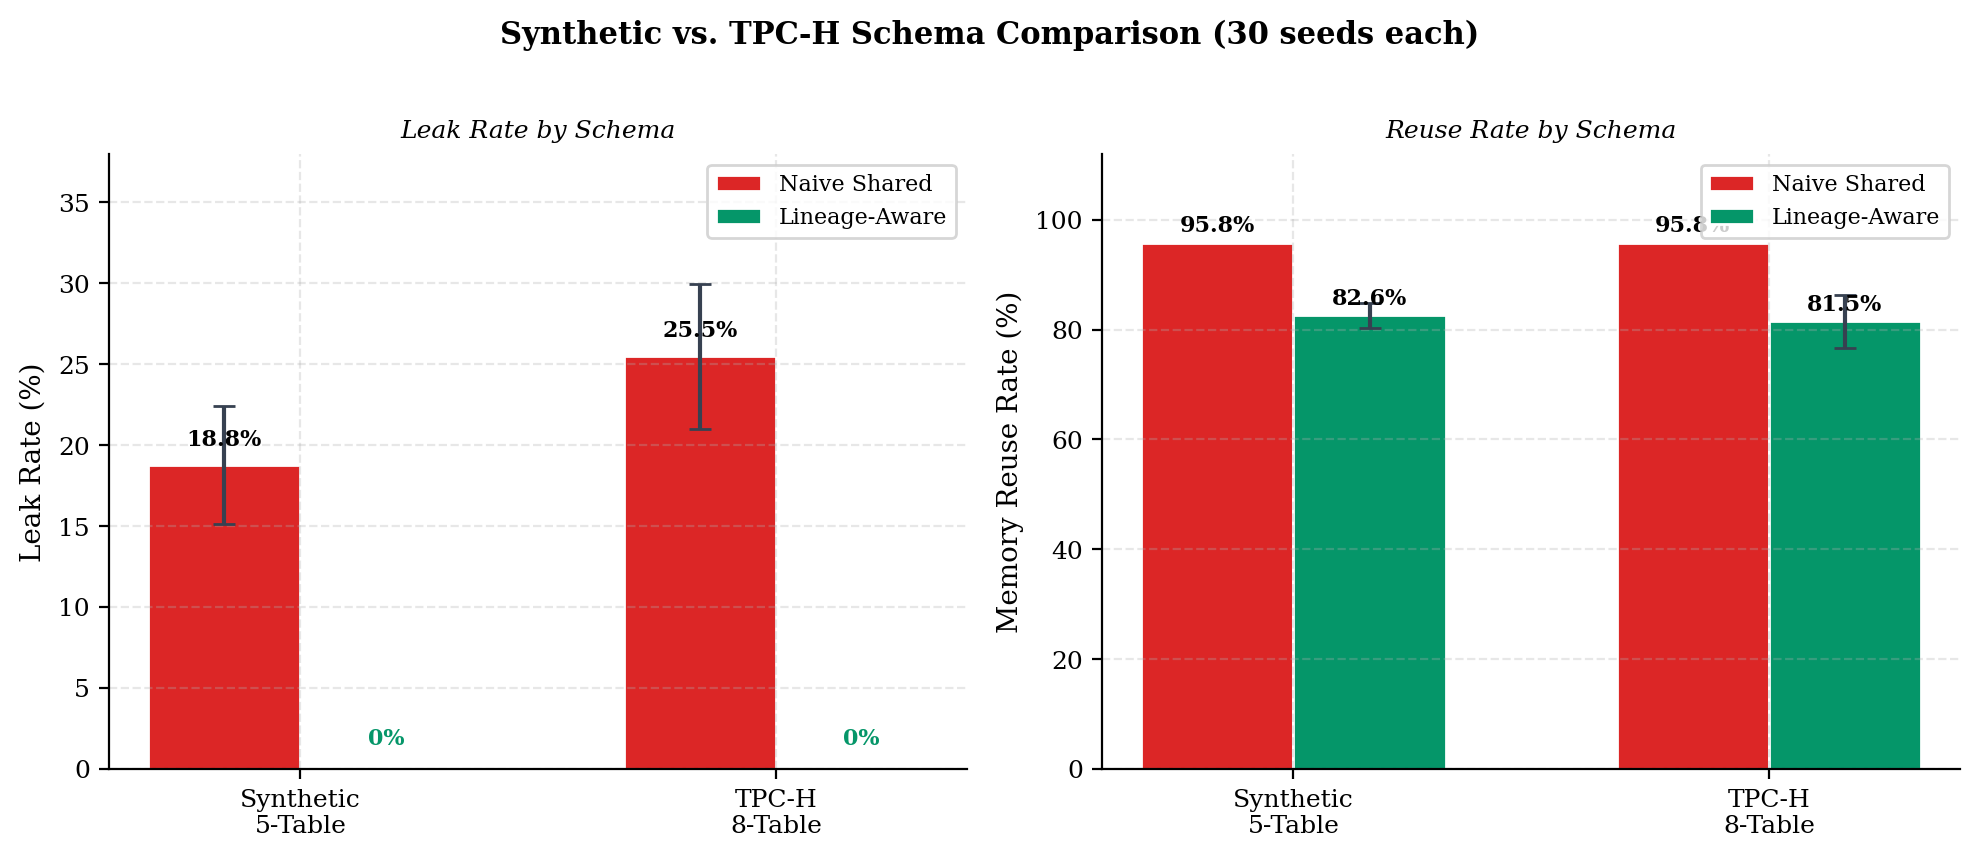
\includegraphics[width=\linewidth]{fig4_tpch_comparison.png}
\caption{Synthetic vs.\ TPC-H schema comparison (30 seeds each). TPC-H's
denser sensitive-column structure yields a higher naive leak rate; lineage-aware
gating eliminates leakage in both configurations.}
\label{fig:tpch}
\end{figure}

The lineage-aware system's $0\%$ leak rate is a \emph{policy guarantee}
(Theorem~\ref{thm:safety}), not an empirical discovery; the substantive
empirical finding is the naive baseline's structurally non-zero leak rate
(effect size $d \approx 7.2$--$8.0$, far beyond the conventional ``large''
threshold of $0.8$), reflecting real retrievals of sensitive-derivation
results by departments that could not have run the underlying queries
themselves.
The governance cost is a $13$--$14$ percentage-point reuse reduction,
i.e., roughly 13 additional query executions per 100 requests---borne as
additional compute, not governance latency, since the gate-check predicate
costs only $0.09\,\mu$s (\S\ref{sec:complexity}).
The consistency of this tradeoff across two substantially different schemas
(60 total seed runs) indicates that content-gated leakage is a structural
property of the failure mode---any workload mixing sensitive and
non-sensitive derivation paths under shared metric names will exhibit it---rather
than an artefact of workload design.
The two schemas differ in sensitive-registry size ($|\mathcal{S}|{=}3$ vs.\
$9$) and join density.
Treating this as a cross-experiment ablation rather than two independent
data points: holding the sensitive-variant proportion constant (2 of 5
metrics in both schemas) while tripling $|\mathcal{S}|$ and increasing join
density corresponds to the leak-rate increase from $18.8\%$ to $25.5\%$,
suggesting leak rate scales with \emph{how many ways} a query can
incidentally touch a sensitive column rather than with how many metrics are
nominally sensitive---consistent with, but not proof of, a monotonic
relationship that a dedicated $2{\times}2{\times}2$ factorial sweep over
step count, registry size, and sensitive-variant proportion (specified in
the Supplementary Material) would establish directly; we list it as the top
empirical priority for follow-on work.

\subsection{Experiment 3: Lineage-Completeness Degradation}
\label{sec:degradation}

Assumption~\ref{ass:complete} is the load-bearing condition of
Theorem~\ref{thm:safety}; in practice agents may under-report lineage due to
bugs or opaque query plans.
We define completeness $\rho \in [0,1]$ as the fraction of each step's
columns correctly reported, and measure the \emph{true} leak rate via a
shadow store that records full ground-truth sensitivity alongside the
truncated lineage the system actually sees.

\begin{figure}[t]
\centering
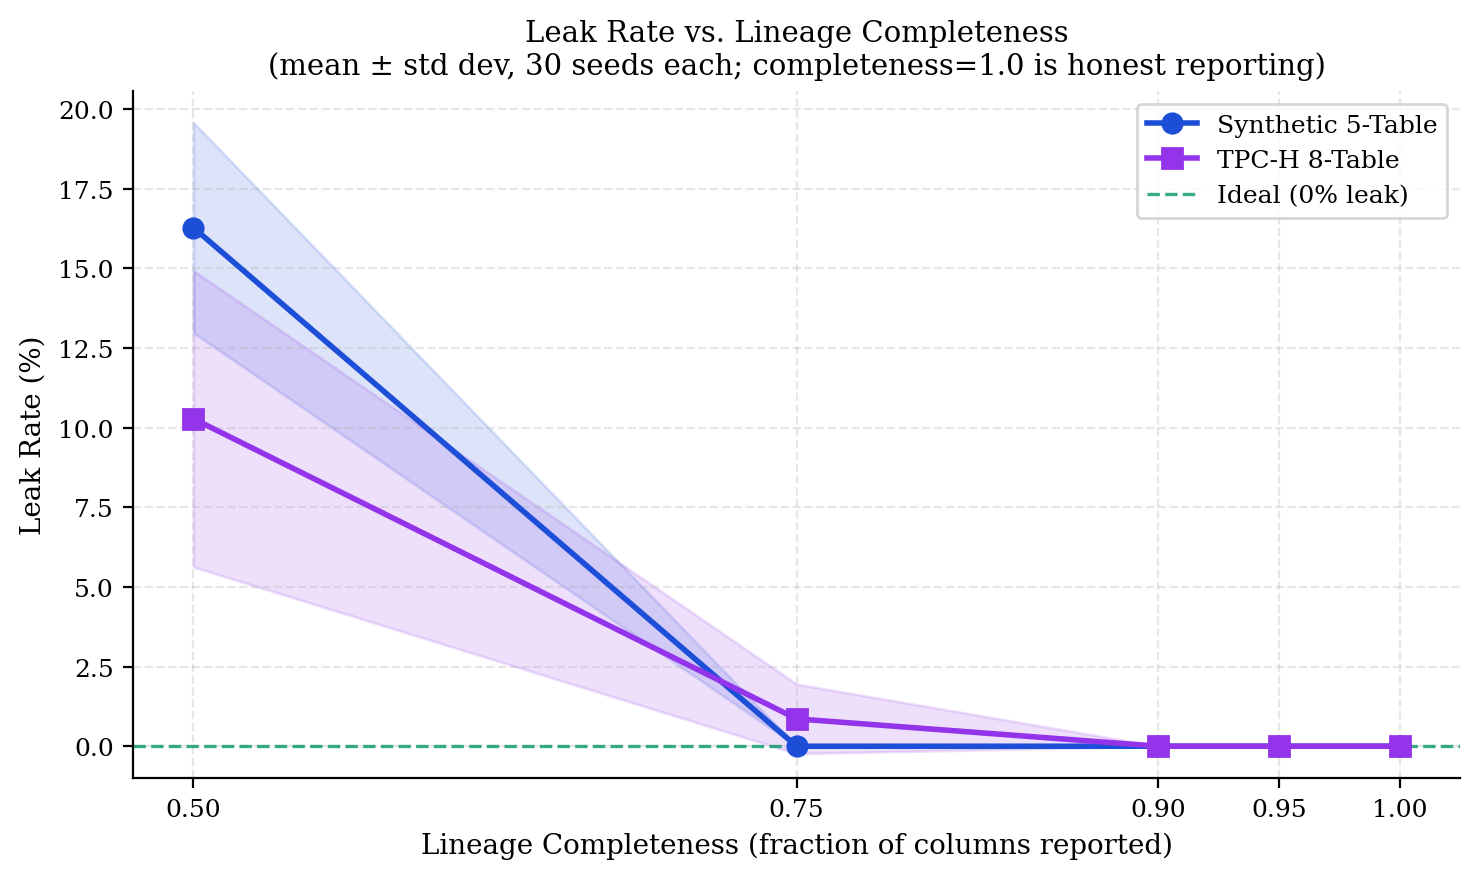
\includegraphics[width=\linewidth]{fig5_degradation.png}
\caption{Leak rate vs.\ lineage completeness $\rho$ (30 seeds, mean
$\pm$1\,std dev shading). Both schemas converge to 0\% by $\rho{=}0.75$--$0.90$;
at $\rho{=}0.50$ the synthetic schema approaches the naive baseline.}
\label{fig:degradation}
\end{figure}

At $\rho{=}0.50$, truncated lineage provides almost no protection (synthetic:
$16.3\pm3.3\%$ leak; TPC-H: $10.3\pm4.7\%$); at $\rho\geq0.75$ (synthetic) or
$\rho\geq0.90$ (TPC-H) the system reaches $0\%$ measured leak rate, converging
on the formal guarantee.
TPC-H needs higher completeness because its sensitive columns spread across
more join steps---join depth is a sensitivity multiplier on the completeness
requirement, not just on raw leak rate.
The actionable recommendation is $\rho \geq 0.9$ as a minimum target,
preferring automatic lineage extraction (Experiment~6) over agent
self-reporting, since the latter is difficult to audit and degrades
unpredictably under exactly the conditions (complex multi-hop joins) where
it matters most.

\subsection{Experiment 4: Extended Fuzzy Conflict-Detection Study}
\label{sec:fuzzy}

The exact-hash detector (Algorithm~\ref{alg:write}) flags any definition-hash
mismatch as a conflict.
We extended an original 10-pair evaluation to 43 hand-labelled lineage pairs
across four categories---15 True Conflicts, 15 Threshold Variants, 8
Logic-Operator changes (AND$\to$OR), and 5 Column-Subset cases---to test
three detectors: D1 (exact hash), D2 (Jaccard filter, $\tau{=}0.70$), and D3
(column-graph).

\begin{table}[t]
\centering
\caption{Extended fuzzy conflict-detection results (43 pairs). Full
per-category breakdown in the Supplementary Material.}
\label{tab:fuzzy}
\footnotesize
\begin{tabular}{@{}lcccc@{}}
\toprule
\textbf{Detector} & \textbf{Prec.} & \textbf{Recall} & \textbf{F\textsubscript{1}} & \textbf{LO correct} \\
\midrule
D1 --- Exact hash          & 0.651 & 1.000 & 0.789 & 8/8 \\
D2 --- Jaccard ($\tau{=}0.70$) & 0.676 & 0.821 & 0.742 & 3/8 \\
D3 --- Column-graph        & \textbf{1.000} & 0.714 & 0.833 & 0/8 \\
\bottomrule
\end{tabular}
\end{table}

The key finding is a previously unreported blind spot: D3, which achieved
perfect $F_1{=}1.00$ on the original 10-pair set, misses all 8
Logic-Operator pairs ($F_1$ drops to $0.833$ on 43 pairs), because it
ignores filter-string variation entirely---correct for threshold
recalibrations, but blind to AND$\to$OR changes that alter metric semantics
without changing the column set.
D1 catches all 8 LO pairs but has weak precision ($0.651$, false-alerting on
every threshold recalibration).
Neither detector alone is production-ready; we propose (but have not
evaluated) a composite D3+filter-logic-structure detector D4, specified in
the Supplementary Material.
This illustrates a general lesson: fuzzy-detection evaluations on small,
narrow datasets can overstate performance by missing edge cases.

\begin{figure}[t]
\centering
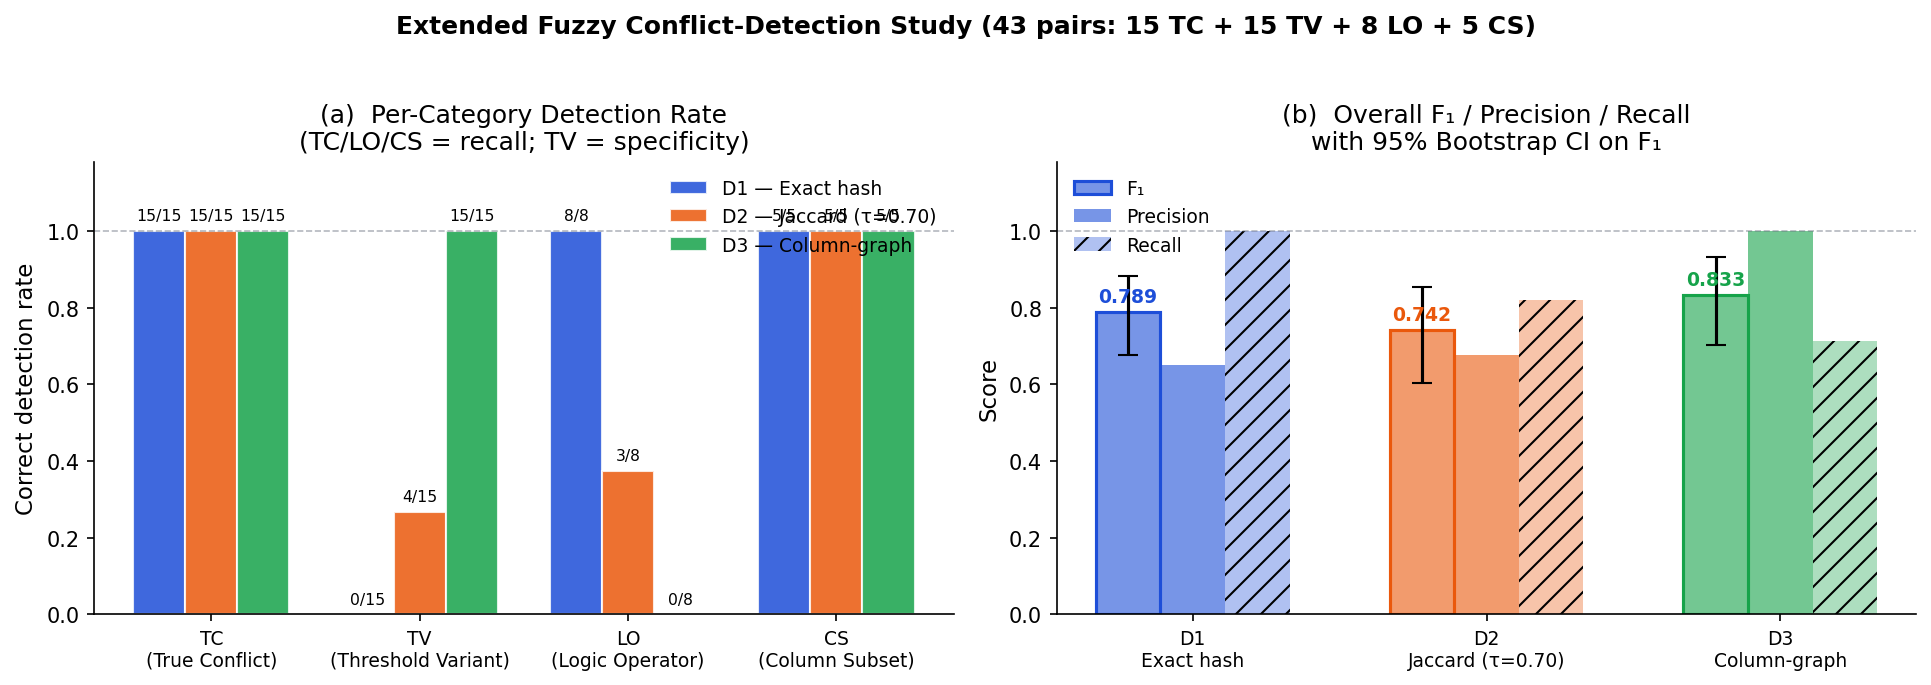
\includegraphics[width=\linewidth]{fig7_fuzzy_extended.png}
\caption{Extended fuzzy conflict-detection results. \textbf{(a)}
Per-category detection rate: recall for TC/LO/CS, specificity for TV. D3's
perfect specificity on TV collapses to zero detection on LO. \textbf{(b)}
Overall $F_1$/precision/recall with 95\% bootstrap CI on $F_1$.}
\label{fig:fuzzy_ext}
\end{figure}

\subsection{Experiment 5: Empirical Runtime Analysis}
\label{sec:runtime}

We instrument all core operations with \texttt{time.perf\_counter()} over
2,000 iterations at five store sizes ($n\in\{1,5,10,20,50\}$), single-threaded
in a standard containerised Python environment with no specialised
acceleration.
\textbf{Hardware and environment:} all measurements were collected on a
4-core Apple Silicon (ARM64) virtual machine with 3.8\,GB RAM, running
Ubuntu~22.04\,LTS (Linux kernel 6.8) and CPython~3.10.12, inside a Docker
container with no GPU, SIMD intrinsics, or JIT acceleration enabled; no other
CPU-bound process ran concurrently during measurement.
We report this configuration in full because the absolute microsecond values
are platform-dependent; the safety-overhead argument in
\S\ref{sec:complexity} relies only on the $O(n)$-vs-$O(1)$ \emph{scaling}
behaviour, which is a property of the algorithm rather than of this specific
machine, but we did not independently re-measure on a second hardware
platform, and we list cross-platform confirmation as a reproducibility item
(\S\ref{sec:futurework}).
Table~\ref{tab:complexity} already reports the key numbers: retrieve
worst-case scales linearly from $0.66\,\mu$s ($n{=}1$) to $13.82\,\mu$s
($n{=}50$), a $21\times$ increase confirming $O(n)$; best-case retrieve and
early-exit conflict detection stay flat, confirming $O(1)$.
Even the worst-case overhead is 2--3 orders of magnitude below typical
production analytics-query latency (single-digit ms to seconds), confirming
the mechanism's practical deployability.
The complete runtime sweep across all five store sizes, including
per-iteration variance, is tabulated in the Supplementary Material.

\subsection{Experiment 6: Real-Agent Integration}
\label{sec:exp6}

Experiments~1--5 assume complete lineage (Assumption~\ref{ass:complete}).
This experiment closes that assumption in practice: we replace agent
self-declared lineage with \emph{automatic} extraction via
\textsc{sqlglot}~\cite{sqlglot2023}, a pure-Python SQL parser, interposed
between the agent and the database cursor---every table and column in the
executed query's abstract syntax tree (AST) is extracted deterministically, so the agent cannot
under-report because it never declares anything.
We use the Northwind database~\cite{northwind2000} with four departments
(Finance, Sales, Operations, HR) and sensitive registry
$\{\texttt{unitprice},\texttt{freight},\texttt{homephone},\texttt{birthdate}\}$,
driven by a LangChain~\cite{langchain2023}+Ollama~\cite{ollama2024} agent
issuing real (and demo-mode canned) SQL across three scenarios covering the
gate's three outcomes: safe reuse, blocked-with-conflict, and vacuous reuse
on a metric with no sensitive columns.

Across all 9 cross-department round-trips, zero sensitive-column leaks
occur: 5 fresh SQL queries are executed and written (2 following a gate
block), 4 requests are served entirely from cache, and 2 gate blocks
precisely coincide with the 2 automatically detected metric-definition
conflicts---i.e., every block corresponded to a genuine semantic divergence,
not a false positive.
Cache-hit latency ($0.009\,$ms) is three to four orders of magnitude below
the SQL it replaces, consistent with the isolated benchmarks of
\S\ref{sec:runtime}.
This small-scale result suggests that automatic SQL lineage extraction can
close Assumption~\ref{ass:complete} for SQL-querying agents in general, with
no change to agent logic and no LLM cooperation required, subject to the
view-, stored-procedure-, and aliasing-related caveats discussed in
\S\ref{sec:discussion} and the larger-scale validation we list as future
work (\S\ref{sec:futurework}).
Full scenario descriptions and the round-trip-by-round-trip table are in the
Supplementary Material.

% =============================================================================
\section{Discussion and Conclusion}
\label{sec:discussion}
% =============================================================================

\subsection{Enterprise Value and What the Experiments Establish}

Three enterprise-facing benefits follow from \S\ref{sec:experiments}.
\emph{Compliance posture}: Theorem~\ref{thm:safety} converts a policy
assertion into a mechanically checkable property that an auditor can verify
by inspecting gate logic rather than trusting agent behaviour, supporting EU
AI Act explainability obligations~\cite{euaiact2024}.
\emph{Avoided breach exposure}: eliminating an $18.8$--$25.5\%$ structural
leak channel is a materially different risk profile given a \$4.44M average
breach cost~\cite{ibm2025breach}.
\emph{Bounded efficiency cost}: the $13$--$14$ point reuse reduction is a
quantified, one-time governance tax rather than an open-ended latency
regression, since the gate itself costs sub-microsecond time.
Taken together, the six experiments show that content-gated memory
systematically leaks across departments (Experiments 1--2); that the
$0\%$ lineage-aware leak rate is a theorem consequence whose real empirical
content is the reuse-cost tradeoff; that the safety guarantee degrades
gracefully rather than catastrophically below full completeness
(Experiment~3); that production conflict detection needs a composite
detector (Experiment~4); that gating overhead is negligible
(Experiment~5); and that automatic SQL lineage extraction closes the
completeness assumption in a real agent stack with zero leaks across 9
real round-trips (Experiment~6).

\subsection{Limitations and Future Work}

\textbf{Limitations:} the $18.8$--$25.5\%$ naive leak rates are properties
of our workload mixes, not universal base rates, though the structural
argument holds independent of any specific percentage; the mechanism does
not catch inference attacks that encode sensitive information in a derived
feature without naming the source column (T4, the most important production
gap); the 43-pair fuzzy dataset remains small; and the runtime benchmarks
(\S\ref{sec:runtime}) were measured on a single hardware/OS configuration,
so the reported constants (though not the $O(n)$-vs-$O(1)$ scaling) may
shift on other platforms.

\textbf{View, stored-procedure, and alias limitations of automatic lineage
extraction.} Experiment 6's automatic-extraction guarantee (closing
Assumption~\ref{ass:complete} without agent cooperation) is only as complete
as \textsc{SQLGlot}'s static AST parse of the executed SQL text. Three
related gaps follow directly from this. First, when a query selects from a
database \emph{view} rather than a base table, \textsc{SQLGlot} records the
view name as the lineage source unless it is also given the view's defining
SQL to expand; if the view definition is not resolved (e.g., it lives only
in the database catalog and was never passed to the extractor), a
sensitive base column hidden behind an innocuously-named view
(\texttt{v\_customer\_summary}) will not appear in $L$, silently violating
Assumption~\ref{ass:complete}. Second, stored procedures and
user-defined functions invoked from SQL (e.g., \texttt{CALL
compute\_churn(...)}) are opaque to AST-level column extraction: the
procedure body may touch sensitive columns internally that never appear as
identifiers in the calling statement, so lineage capture requires either
inlining the procedure body ahead of parsing or maintaining a separate
column-level lineage annotation for each registered procedure. Third,
column and table \emph{aliasing} (\texttt{SELECT c.income AS c1}, or
self-joins that alias the same physical table twice) is generally resolved
correctly by \textsc{SQLGlot}'s scope analysis, but deeply nested aliasing
across multiple levels of subquery or common table expression (CTE) can defeat resolution in
practice, particularly when combined with \texttt{SELECT~*} expansion
against a catalog the extractor was not given.
In all three cases the system's fail-closed design
(\S\ref{sec:implementation}) bounds the damage to over-blocking (an AMU
that should have been retrievable is marked maximally sensitive) rather
than leakage, but this is a completeness gap in Experiment 6's zero-leak
result that a purely syntactic extractor cannot close without
catalog-aware view/procedure expansion---an engineering extension we flag
as future work below rather than something the current implementation
does.

\textbf{Future work, in priority order:}\label{sec:futurework}
(1)~adversarial lineage testing---red-team
queries that smuggle sensitive joins through derived features or
view indirection, stress-testing Assumption~\ref{ass:complete}; (2)~non-SQL
lineage extraction for vector-store, REST/GraphQL, and in-process
derivations, and catalog-aware view/stored-procedure expansion for the SQL
case; (3)~a production deployment study on a real 20--50 table
warehouse over weeks rather than seeds, on more than one hardware platform;
and (4)~implementing and evaluating
the proposed D4 composite conflict detector against a larger real-analytics
corpus, alongside open-sourcing the reference implementation.

\subsection{Conclusion}

Every current AI agent memory system governs \emph{what} is stored and
\emph{who} may access it, but not \emph{how} the stored result was derived.
The Analytical Memory Unit schema and lineage-gated retrieval policy close
this gap at minimal overhead---$4$--$8\times$ storage, a sub-microsecond
gate check, and at most $13.8\,\mu$s worst-case retrieval latency---with a
formal safety guarantee (Theorem~\ref{thm:safety}) and six experiments
characterising its behaviour, degradation, and real-agent viability.
As AI agents move from single-purpose assistants to interconnected
participants in enterprise data workflows, the systems that govern what
those agents remember will increasingly determine what those agents are
permitted to say, and to whom; content-and-role governance answers ``who
owns this memory,'' while derivation-gated governance answers the equally
necessary question, ``could this requester have produced this result
themselves.''

% =============================================================================
\section{Reproducibility, Data, and Ethics}
\label{sec:repro}
% =============================================================================

The reference implementation (Python; AMU/lineage data model, three
competing memory systems, event-replay simulator, statistical analysis, and
the \textsc{sqlglot}-based real-agent pipeline) reproduces every table and
figure in this paper and is containerised via Docker Compose for
one-command reproduction; full module-by-module documentation is in the
Supplementary Material.
No proprietary or personally identifiable data was used: the synthetic and
TPC-H-inspired schemas use generated or benchmark data, and the Northwind
database (Experiment~6) is a decades-old public fictional dataset
containing no real individuals' information.
This work does not involve human subjects or data requiring ethical review.
The threat model (\S\ref{sec:threat}) is deliberately explicit about what
the mechanism does \emph{not} protect against, because overstating a safety
guarantee's scope is itself a governance risk.
Source code, generated datasets, and raw per-seed results will be made
available at a public repository upon acceptance, and are available from
the corresponding author upon reasonable request in the interim.

% =============================================================================
\section*{Conflict of Interest}
The authors declare that they have no known competing financial interests
or personal relationships that could have appeared to influence the work
reported in this paper.

\section*{Acknowledgment}
This research received no specific grant from any funding agency in the
public, commercial, or not-for-profit sectors. The authors thank no
additional contributors beyond those listed in the author list.

% =============================================================================
\balance
\begin{thebibliography}{28}

\bibitem{digitalapplied2026adoption}
Digital Applied, ``AI agent adoption 2026: 120+ enterprise data points,''
Digital Applied, Tech. Rep., 2026, aggregating Gartner and S\&P Global
Market Intelligence/McKinsey survey data. [Online]. Available:
\url{https://www.digitalapplied.com/blog/ai-agent-adoption-2026-enterprise-data-points}

\bibitem{ibm2025breach}
IBM Security, ``Cost of a data breach report 2025,'' IBM, Tech. Rep., 2025.
[Online]. Available: \url{https://www.ibm.com/reports/data-breach}

\bibitem{elyagoubi2026agentleak}
F. El Yagoubi, G. Badu-Marfo, and R. Al Mallah, ``AgentLeak: A full-stack
benchmark for privacy leakage in multi-agent LLM systems,'' \emph{arXiv
preprint arXiv:2602.11510}, 2026.

\bibitem{packer2023memgpt}
C. Packer, S. Wooders, K. Lin, V. Fang, S. G. Patil, I. Stoica, and
J. E. Gonzalez, ``MemGPT: Towards LLMs as operating systems,''
\emph{arXiv preprint arXiv:2310.08560}, 2023.

\bibitem{rasmussen2025zep}
P. Rasmussen, ``Zep: A temporal knowledge graph architecture for agent
memory,'' \emph{arXiv preprint arXiv:2501.13956}, 2025.

\bibitem{xu2025amem}
W. Xu, Z. Liang, K. Mei, H. Gao, J. Tan, and Y. Zhang, ``A-MEM: Agentic
memory for LLM agents,'' in \emph{Proc. Adv. Neural Inf. Process. Syst.
(NeurIPS)}, 2025, arXiv:2502.12110.

\bibitem{taheri2026governed}
H. Taheri, ``Governed memory: A production architecture for multi-agent
workflows,'' \emph{arXiv preprint arXiv:2603.17787}, 2026.

\bibitem{lam2026ssgm}
C. Lam, J. Li, L. Zhang, and K. Zhao, ``Governing evolving memory in LLM
agents: Risks, mechanisms, and the stability and safety governed memory
(SSGM) framework,'' \emph{arXiv preprint arXiv:2603.11768}, 2026.

\bibitem{oracle2026memory}
Oracle Corporation, ``Oracle AI agent memory: A governed, unified memory
core for enterprise AI agents,'' Oracle Developer Blog, Mar. 2026.
[Online]. Available:
\url{https://blogs.oracle.com/developers/oracle-ai-agent-memory-a-governed-unified-memory-core-for-enterprise-ai-agents}

\bibitem{colrows2024metrics}
Colrows, ``Why BI metrics do not match across dashboards,'' Colrows
Technical Blog, 2024. [Online]. Available:
\url{https://colrows.com/blogs/why-bi-metrics-do-not-match-across-dashboards/}

\bibitem{snowflake2025osi}
Snowflake, Salesforce, dbt Labs, BlackRock, and RelationalAI, ``Open
Semantic Interchange (OSI): A vendor-neutral semantic layer specification
for AI and BI,'' Industry Standard Initiative, Sep. 2025. [Online].
Available:
\url{https://www.snowflake.com/en/news/press-releases/snowflake-salesforce-dbt-labs-and-more-revolutionize-data-readiness-for-ai-with-open-semantic-interchange-initiative/}

\bibitem{euaiact2024}
European Parliament and Council, ``Regulation (EU) 2024/1689 laying down
harmonised rules on artificial intelligence (EU AI Act),'' Official
Journal of the European Union, Jul. 2024. [Online]. Available:
\url{https://eur-lex.europa.eu/legal-content/EN/TXT/?uri=CELEX:32024R1689}

\bibitem{du2026survey}
P. Du, ``Memory for autonomous LLM agents: Mechanisms, evaluation, and
emerging frontiers,'' \emph{arXiv preprint arXiv:2603.07670}, 2026.

\bibitem{abaev2026agentguardian}
N. Abaev, D. Klimov, G. Levinov, D. Mimran, Y. Elovici, and A. Shabtai,
``AgentGuardian: Learning access control policies to govern AI agent
behavior,'' \emph{arXiv preprint arXiv:2601.10440}, 2026.

\bibitem{subramaniam2024deploi}
P. Subramaniam and S. Krishnan, ``DePLOI: Applying NL2SQL to synthesize
and audit database access control,'' \emph{arXiv preprint
arXiv:2402.07332}, 2024.

\bibitem{moreau2011prov}
L. Moreau, B. Clifford, J. Freire, J. Futrelle, Y. Gil, P. Groth,
N. Kwasnikowska, S. Miles, P. Missier, J. Myers, B. Plale, Y. Simmhan,
E. Stephan, and J. Van den Bussche, ``The open provenance model---core
specification (v1.1),'' \emph{Future Gener. Comput. Syst.}, vol. 27,
no. 6, pp. 743--756, 2011, doi: 10.1016/j.future.2010.07.005. See also
W3C PROV-DM: \url{https://www.w3.org/TR/prov-dm/}.

\bibitem{herschel2017survey}
M. Herschel, R. Diestelk\"{a}mper, and H. Ben Lahmar, ``A survey on
provenance: What for? What form? What from?,'' \emph{The VLDB J.},
vol. 26, no. 6, pp. 881--906, 2017, doi: 10.1007/s00778-017-0486-1.

\bibitem{zhang2025lineagex}
S. H. Zhang, Z. Miao, and J. Wang, ``LINEAGEX: A column lineage
extraction system for SQL,'' in \emph{Proc. 41st IEEE Int. Conf. Data
Eng. (ICDE), Demo Track}, 2025, arXiv:2505.23133.

\bibitem{naik2026omnileak}
A. Naik, J. Culligan, Y. Gal, P. Torr, R. Aljundi, A. Paren, and A. Bibi,
``OMNI-LEAK: Orchestrator multi-agent network induced data leakage,''
\emph{arXiv preprint arXiv:2602.13477}, 2026.

\bibitem{alizadeh2025leak}
M. Alizadeh, Z. Samei, D. Stetsenko, and F. Gilardi, ``Simple prompt
injection attacks can leak personal data observed by LLM agents during
task execution,'' \emph{arXiv preprint arXiv:2506.01055}, 2025.

\bibitem{wang2026authgraph}
P. Wang, Y. Li, and Y. Tian, ``Aligning provenance with authorization: A
dual-graph defense for LLM agents,'' \emph{arXiv preprint
arXiv:2605.26497}, 2026.

\bibitem{tpch2021}
Transaction Processing Performance Council, \emph{TPC-H Benchmark
Specification, Revision 3.0.1}. TPC, 2021. [Online]. Available:
\url{http://www.tpc.org/tpch/}

\bibitem{sqlglot2023}
T. Mao and contributors, ``sqlglot: SQL parser and transpiler,'' 2023,
MIT Licence, version 23+ used in this work. [Online]. Available:
\url{https://github.com/tobymao/sqlglot}

\bibitem{northwind2000}
Microsoft Corporation, \emph{Northwind Traders Sample Database}, 2000,
canonical fictional business dataset. [Online]. Available (open-source
SQLite port): \url{https://github.com/jpwhite3/northwind-SQLite3}

\bibitem{langchain2023}
H. Chase and contributors, ``LangChain: Building applications with LLMs
through composability,'' 2023, MIT Licence. [Online]. Available:
\url{https://github.com/langchain-ai/langchain}

\bibitem{ollama2024}
Ollama contributors, ``Ollama: Run LLMs locally,'' 2024, MIT Licence,
local LLM server used in Experiment~6. [Online]. Available:
\url{https://github.com/ollama/ollama}

\bibitem{rezazadeh2025collabmem}
A. Rezazadeh, Z. Li, A. Lou, Y. Zhao, W. Wei, and Y. Bao, ``Collaborative
memory: Multi-user memory sharing in LLM agents with dynamic access
control,'' \emph{arXiv preprint arXiv:2505.18279}, 2025.

\bibitem{ren2026gatemem}
Z. Ren, Y. Yang, Y. Chen, Z. Zhao, B. Fu, Z. Shu, B. Zhang, Y. Xu, D. Guo,
and S. Yan, ``GateMem: Benchmarking memory governance in multi-principal
shared-memory agents,'' \emph{arXiv preprint arXiv:2606.18829}, 2026.

\end{thebibliography}

\vspace{6pt}

\begin{IEEEbiographynophoto}{Venkata Sangaraju}
is an independent researcher working on memory and data-governance
architectures for enterprise artificial intelligence (AI) agents. His
research interests include lineage and provenance tracking for AI agent
systems, privacy-preserving retrieval, column-level access control, and the
application of formal safety guarantees to shared multi-agent memory
infrastructure. He is the corresponding author of this work
(ORCID: 0009-0001-7716-1342).
\end{IEEEbiographynophoto}

\begin{IEEEbiographynophoto}{Sudhir Vissa}
is with SAGE7 AI, Georgetown, Texas, USA. His research interests include
enterprise AI agent architectures, data governance, and applied
infrastructure for multi-agent deployments, including the
metric-definition and access-control problems addressed in this work
(ORCID: 0009-0003-7865-0863).
\end{IEEEbiographynophoto}
\EOD

\end{document}
